% IPMI Figure 1

\begin{figure}
\centering
\begin{tabular}{c c c c}
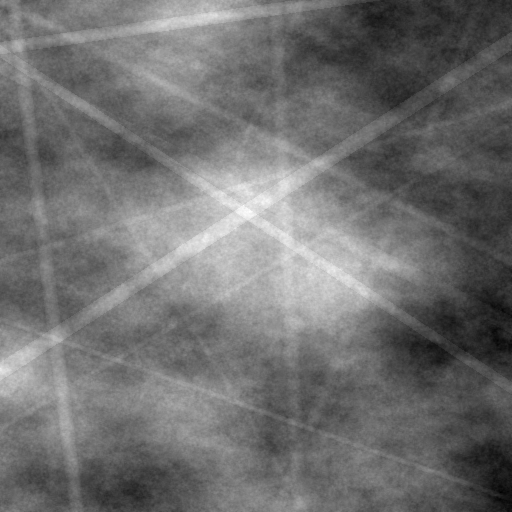
\includegraphics[width=\qtrcol]{\figpath/ipmi/line512_003} &
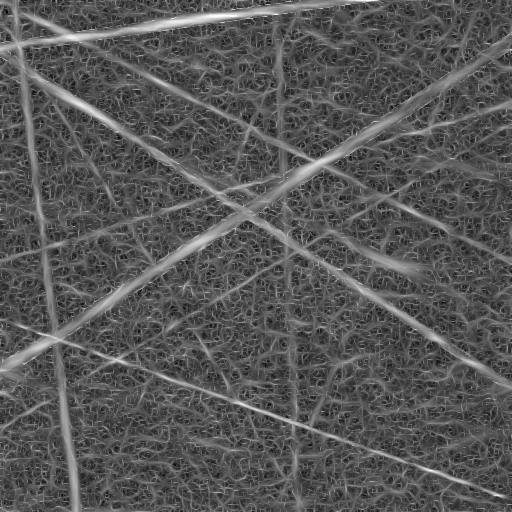
\includegraphics[width=\qtrcol]{\figpath/ipmi/line512_003_lines} &
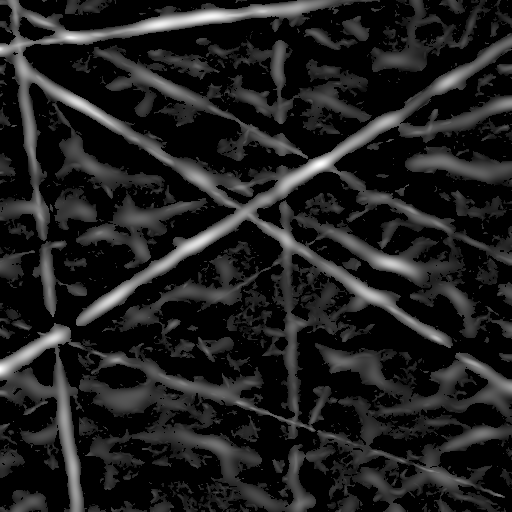
\includegraphics[width=\qtrcol]{\figpath/ipmi/line512_003_gaussian} &
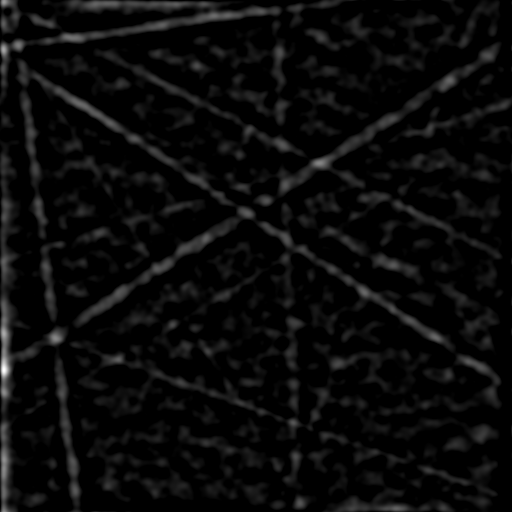
\includegraphics[width=\qtrcol]{\figpath/ipmi/line512_003_monogenic} \\
(a) & (b) & (c) & (d) \\
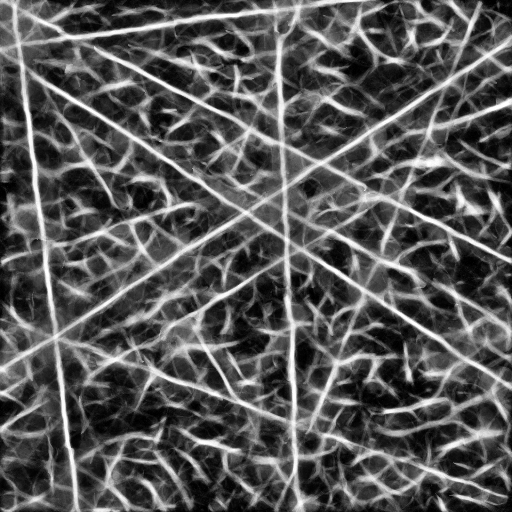
\includegraphics[width=\qtrcol]{\figpath/ipmi/line512_003_rf_191905} &
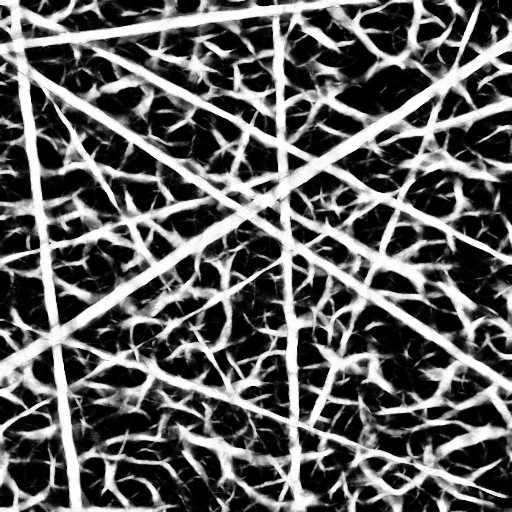
\includegraphics[width=\qtrcol]{\figpath/ipmi/line512_003_rf_191961} &
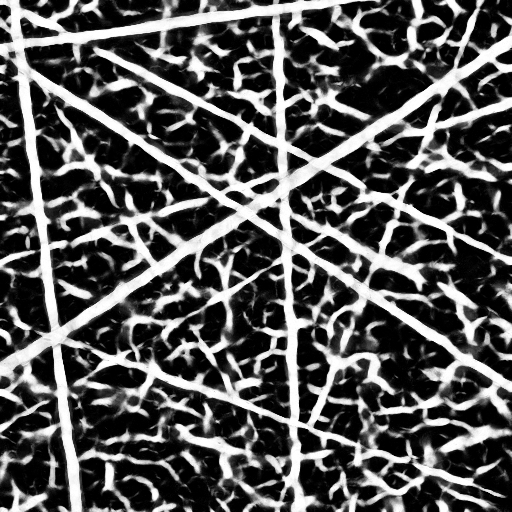
\includegraphics[width=\qtrcol]{\figpath/ipmi/line512_003_rf_233141} &
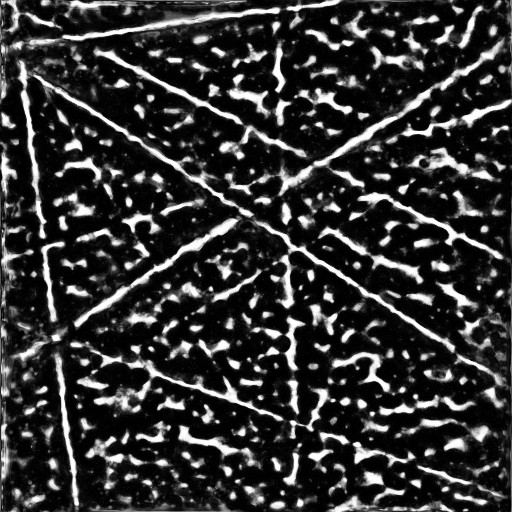
\includegraphics[width=\qtrcol]{\figpath/ipmi/line512_003_rf_191960} \\
(e) & (f) & (g) & (h)
\end{tabular}
%
\caption{Synthetic test image and corresponding filter responses: (a) original image; (b) Linop; (c) Gaussian; (d) Monogenic; (e) DT-CWT/RF; (f) Linop/RF; (g) Gaussian/RF; (h) Monogenic/RF.}
\label{f:synthetic_responses}
\end{figure}